\textbf{{1.二进制、八进制、十进制、十六进制的基本概念}}

\textbf{十进制:}日常生活中的进位计数制都是十进制。

\textbf{二进制:}二进制是计算技术中使用最广泛的一种数制,使用0和1两个数码来表示。

\textbf{八进制和十六进制:}规则和二进制相似。

\textbf{{2.二进制、八进制、十进制、十六进制的相互转换}}

二进制、八进制、十六进制转换为十进制:仅以二进制转换为十进制为例,八进制和十六进制转换为十进制的方法是一样的,只需调整每一位的权重即可。

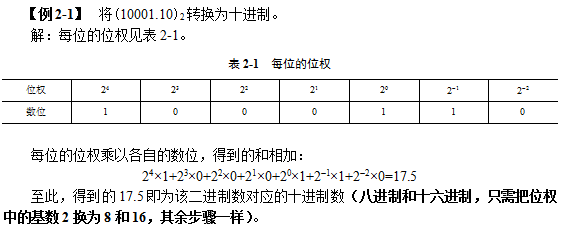
\includegraphics[width=3.70833in,height=1.51042in]{png-jpeg-pics/7EDEFAD7FA51962C5B15F65354D73BB4.png}

十进制转换为二进制、八进制、十六进制:这里仍然以十进制转换为二进制为例。

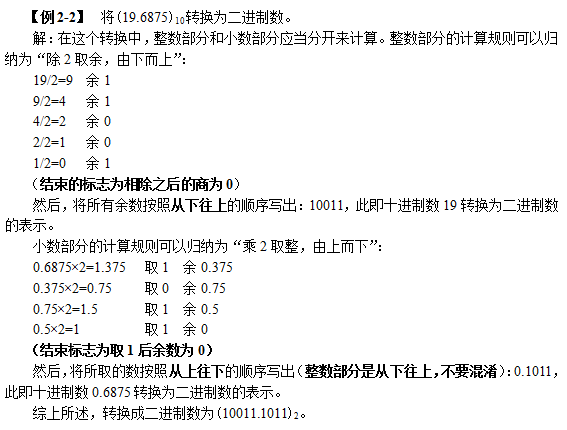
\includegraphics[width=3.70833in,height=2.81250in]{png-jpeg-pics/E6B48075C7E26FC3D268151E18A67A21.png}
